%%%%%%%%%%%%%%%%%%%%%PREAMBLE BEGINS%%%%%%%%%%
\documentclass [serif,professionalfont]{beamer}
\usepackage [T1]{fontenc} % Needed for Type1 Concrete
\usepackage {concrete}
\usepackage[utf8]{inputenc}
\usepackage{fontawesome,tikz,amsmath,amssymb,graphicx,wrapfig,hyperref,mathtools,multirow,tabularx,mathtools}
\usepackage[normalem]{ulem}%for strikethrough
\usepackage[symbol]{footmisc}%for footnote symbols
\renewcommand{\thefootnote}{\fnsymbol{footnote}}
\usepackage{adjustbox,comment,appendixnumberbeamer}
\usetikzlibrary{petri,automata,positioning,arrows,fit,shapes}
\usetikzlibrary{positioning,shapes.callouts}
\usepackage{rotating}
\useinnertheme{rectangles}%itemized bullets as rectangles
\newcommand{\Lstar}{$\mathcal{L}_{UCS}^{1}$}
\newcommand*{\eqdef}{\stackrel{\text{def}}{=}}
\newcommand{\iCar}{\raisebox{-0.9\height}{\faCar}}
%\logo{\includegraphics[width=1cm]{figures/IITDhL}}
\beamertemplatenavigationsymbolsempty
\setbeamertemplate{footline}[frame number]
\tikzstyle{aldecision} = [diamond, draw, fill=blue!20,
text width=4.5em, text badly centered, node distance=2.5cm, inner sep=0pt]
\tikzstyle{alblock} = [rectangle, draw, fill=blue!20,
text width=5em, text centered, rounded corners, minimum height=4em]
\tikzstyle{line} = [draw, very thick, color=black!50, -latex']
\tikzstyle{allibrary} = [draw, ellipse,fill=red!20, node distance=2.5cm,
minimum height=2em]
%for live windows
\usepackage{pgfgantt}
\definecolor{foobarblue}{RGB}{0,153,255}
\newganttchartelement{foobar}{
foobar/.style={
shape=rectangle,
inner sep=0pt,
draw=foobarblue!50!black,
very thick,
fill=white
}
}
\newcommand\textganttbar[4]{%
    \ganttfoobar{#1}{#3}{#4}
    \ganttfoobar[inline,bar label font=\footnotesize]
    {#2}{#3}{#4}
}
%\setbeamertemplate{blocks}[rounded][shadow=true]
%\setbeamercolor{block body}{bg=cyan!10}
\newcommand{\hlfancy}[2]{\sethlcolor{#1}\hl{#2}}
%%%%%%%%%%%%%%%%%%%%%%%%%%%%%%%%%%%%%%%%%%%%%%%%%%%%%%%%%%%%%%%%

\title{$\mathcal{L}_{UCS}^{1}$: A \textcolor{purple}{Monodic} Logic for Bounded Model Checking of \textcolor{purple}{Unbounded Client-Server Systems}}

\author{\small{Ramchandra Phawade\inst{1}\and
\underline{Tephilla Prince}\inst{1}\and
S. Sheerazuddin\inst{2}}} 
\institute{Indian Institute of Technology Dharwad, India \and
National Institute of Technology Calicut, India \\
} 

%\institute{\vspace{-2em}ICLA 2023}
\date{\tiny{3/3/2023}\\ICLA'23, IIT Indore}
%\usepackage[style=verbose]{bibtex}
%\bibliographystyle{plain}
\usepackage[style=authortitle,backend=bibtex]{biblatex}
\bibliography{mybibliography.bib}
\renewbibmacro*{cite:title}{%
  \printtext[bibhyperref]{%
    \printfield[citetitle]{labeltitle}%
    \setunit{\space}%
    \printtext[parens]{\printdate}%
  }%
}
%%%%%%%%%%%%%%%%%%%%%PREAMBLE ENDS%%%%%%%%%%%%


\begin{document}

\begin{frame}
\titlepage
\end{frame}


%Autonomous Parking System
\begin{frame}
\frametitle{A toy example}
%\centering

    \begin{tikzpicture}[scale=0.45, note/.style={rectangle callout, fill=####1}]
\visible<1>{

\node[draw,text width=5cm, draw=green!15, fill=green!15] at (13,12) {An empty Parking Lot waits for vehicles};
}       
        \node   at  (1,1)   [rectangle, thick, draw=yellow!20, fill=black!30,inner sep=0pt,minimum height=4cm, minimum width=5.5cm] (bga){};
        %Row0
        \node   at  (5,3.5)     [rectangle, thick, draw=yellow!90, fill=black!5,inner sep=0pt,minimum height=1cm, minimum width=0.8cm] (s1){};
        
        \node   at  (2.5,3.5)   [rectangle, thick, draw=yellow!90, fill=black!5,inner sep=0pt,minimum height=1cm, minimum width=0.8cm] (s2){};
        
        \node   at  (0,3.5)     [rectangle, thick, draw=yellow!90, fill=black!5,inner sep=0pt,minimum height=1cm, minimum width=0.8cm] (s3){};
        
        \node   at  (-2.5,3.5)  [rectangle, thick, draw=yellow!90, fill=black!5,inner sep=0pt,minimum height=1cm, minimum width=0.8cm] (s4){};
        
        %closed gate
        \node   at  (6.6,1.8)   [rectangle, thick, draw=green!90, fill=black!60,inner sep=0pt,minimum height=1cm, minimum width=0.2cm] (gate){};
        
        
        %Row1
        \node   at  (5,-0.5)    [rectangle, thick, draw=yellow!90, fill=black!5,inner sep=0pt,minimum height=1cm, minimum width=0.8cm] (s5){};
        
        \node   at  (2.5,-0.5)  [rectangle, thick, draw=yellow!90, fill=black!5,inner sep=0pt,minimum height=1cm, minimum width=0.8cm] (s6){};
        
        \node   at  (0,-0.5)    [rectangle, thick, draw=yellow!90, fill=black!5,inner sep=0pt,minimum height=1cm, minimum width=0.8cm] (s7){};
        
        \node   at  (-2.5,-0.5)     [rectangle, thick, draw=yellow!90, fill=black!5,inner sep=0pt,minimum height=1cm, minimum width=0.8cm] (s8){};
        
        \node   at  (6,7.5)     [circle, thick, draw=red!50,inner sep=0pt,minimum height=1cm, minimum width=1cm] (parking){\large P};
        
        \node   at  (6,5.5)     [rectangle, thick, draw=red!50,inner sep=0pt,minimum height=-.2cm, minimum width=0.2cm] (hidden){};
        
        \draw (parking) -- (hidden);
        
        
%car outside gate       
\visible<2,3>{      
        \node   at  (8,1.8)     [rectangle, thick,inner sep=0pt,minimum height=1cm, minimum width=0.2cm] (car){{\iCar}1};
}
%Park Request
\visible<2>{        
         \node [note=yellow!50, callout absolute pointer={(8,2)}] at (12,4) {Can I park here?};
}

%Accept request      
\visible<3>{
 \node [note=blue!20, callout absolute pointer={(6,6)}] at (12,4){Yeah, come in!};
 \node  at  (6.6,1.8)   [rectangle, thick, draw=green!30, fill=green!30,inner sep=0pt,minimum height=1cm, minimum width=0.2cm] (gate){};}

%Allocated Parking Lot       
\visible<4>{
  \node     at  (5,3.5)     [rectangle, thick, draw=yellow!90, fill=black!5,inner sep=0pt,minimum height=1cm, minimum width=0.8cm] (s1){\iCar 1};
 \node [note=blue!20, callout absolute pointer={(6,6)}] at (12,4){Parking Lot allocated};
}   

%Multiple Requests waiting
\visible<5>{        %car outside gate

\node[draw,text width=4cm, draw=green!15, fill=green!15] at (13,12) {Unbounded number of parking requests};

 \node  at  (5,3.5)     [rectangle, thick, draw=yellow!90, fill=black!5,inner sep=0pt,minimum height=1cm, minimum width=0.8cm] (s1){\iCar 1};
        \node   at  (8,1.8)     [rectangle, thick,inner sep=0pt,minimum height=1cm, minimum width=0.2cm] (car1){\iCar 2};
        \node   at  (10,1.8)    [rectangle, thick,inner sep=0pt,minimum height=1cm, minimum width=0.2cm] (car2){\iCar 3};
        \node   at  (12,1.8)    [rectangle, thick,inner sep=0pt,minimum height=1cm, minimum width=0.2cm] (car3){\iCar 4};
        \node   at  (14,1.8)    [rectangle, thick,inner sep=0pt,minimum height=1cm, minimum width=0.2cm] (car4){\iCar 5};
        
        \node   at  (16,1.8)    [rectangle, thick,inner sep=0pt,minimum height=1cm, minimum width=0.2cm] (car1){$\ldots$};
        %\node   at  (18,1.8)    [rectangle, thick,inner sep=0pt,minimum height=1cm, minimum width=0.2cm] (car2){\faCar};
        %\node   at  (20,1.8)    [rectangle, thick,inner sep=0pt,minimum height=1cm, minimum width=0.2cm] (car3){\faCar};
        
         \node [note=yellow!50, callout absolute pointer={(8,2)}] at (12,4) {Can I park here?};
}

\visible<6>{

\node[draw,text width=3cm, draw=green!15, fill=green!15] at (13,12) {No parking space};

}    
     
%Parking lot full
\visible<6,7,8,9>{
%Row0
        \node   at  (5,3.5)     [rectangle, thick, draw=yellow!90, fill=black!5,inner sep=0pt,minimum height=1cm, minimum width=0.8cm] (s1){\iCar 1};
        
        \node   at  (2.5,3.5)   [rectangle, thick, draw=yellow!90, fill=black!5,inner sep=0pt,minimum height=1cm, minimum width=0.8cm] (s2){\iCar 3};
        
        \node   at  (0,3.5)     [rectangle, thick, draw=yellow!90, fill=black!5,inner sep=0pt,minimum height=1cm, minimum width=0.8cm] (s3){\iCar 98};
        
        \node   at  (-2.5,3.5)  [rectangle, thick, draw=yellow!90, fill=black!5,inner sep=0pt,minimum height=1cm, minimum width=0.8cm] (s4){\iCar 2};    
                
        
        %Row1
        \node   at  (5,-0.5)    [rectangle, thick, draw=yellow!90, fill=black!5,inner sep=0pt,minimum height=1cm, minimum width=0.8cm] (s5){\iCar 10};
        
        \node   at  (2.5,-0.5)  [rectangle, thick, draw=yellow!90, fill=black!5,inner sep=0pt,minimum height=1cm, minimum width=0.8cm] (s6){\iCar 23};
        
        \node   at  (0,-0.5)    [rectangle, thick, draw=yellow!90, fill=black!5,inner sep=0pt,minimum height=1cm, minimum width=0.8cm] (s7){\iCar 11};
        
        \node   at  (-2.5,-0.5)     [rectangle, thick, draw=yellow!90, fill=black!5,inner sep=0pt,minimum height=1cm, minimum width=0.8cm] (s8){\iCar 94};
        
}

%Request when Full
\visible<7>{

\node   at  (8,1.8)     [rectangle, thick,inner sep=0pt,minimum height=1cm, minimum width=0.2cm] (car){\iCar 99};
\node [note=yellow!50, callout absolute pointer={(8,2.5)}] at (12,4) {Can I park here?};

}    
     
%Reject request when full
\visible<8>{
\node [note=blue!20, callout absolute pointer={(6,6)}] at (12,4){No};
\node   at  (6.6,1.8)   [rectangle, thick, draw=red!30, fill=red!30,inner sep=0pt,minimum height=1cm, minimum width=0.2cm] (gate){};
\node   at  (8,1.8)     [rectangle, thick,inner sep=0pt,minimum height=1cm, minimum width=0.2cm] (car){\iCar 99};      
}

%Vehicle Exit Request
\visible<9>{
%        \node  at  (5,3.5)     [rectangle, thick, draw=yellow!90, fill=black!5,inner sep=0pt,minimum height=1cm, minimum width=0.5cm] (s1){\iCar 1};
        \node [note=yellow!50, callout absolute pointer={(5,3.5)}] at (12,4) {I'm exiting};

}
%Deallocate Parking lot 
\visible<10>{
 \node [note=blue!20, callout absolute pointer={(6,6)}] at (12,4){Parking Lot Deallocated};
        \node   at  (5,3.5)     [rectangle, thick, draw=yellow!90, fill=black!5,inner sep=0pt,minimum height=1cm, minimum width=0.8cm] (s1){};
        
        \node   at  (2.5,3.5)   [rectangle, thick, draw=yellow!90, fill=black!5,inner sep=0pt,minimum height=1cm, minimum width=0.8cm] (s2){\iCar 3};
        
        \node   at  (0,3.5)     [rectangle, thick, draw=yellow!90, fill=black!5,inner sep=0pt,minimum height=1cm, minimum width=0.8cm] (s3){\iCar 98};
        
        \node   at  (-2.5,3.5)  [rectangle, thick, draw=yellow!90, fill=black!5,inner sep=0pt,minimum height=1cm, minimum width=0.8cm] (s4){\iCar 2};    
                
        
        %Row1
        \node   at  (5,-0.5)    [rectangle, thick, draw=yellow!90, fill=black!5,inner sep=0pt,minimum height=1cm, minimum width=0.8cm] (s5){\iCar 10};
        
        \node   at  (2.5,-0.5)  [rectangle, thick, draw=yellow!90, fill=black!5,inner sep=0pt,minimum height=1cm, minimum width=0.8cm] (s6){\iCar 23};
        
        \node   at  (0,-0.5)    [rectangle, thick, draw=yellow!90, fill=black!5,inner sep=0pt,minimum height=1cm, minimum width=0.8cm] (s7){\iCar 11};
        
        \node   at  (-2.5,-0.5)     [rectangle, thick, draw=yellow!90, fill=black!5,inner sep=0pt,minimum height=1cm, minimum width=0.8cm] (s8){\iCar 94};
}

%Vehicle Request to exit and incoming parking request.
\visible<11>{
%\frametitle{A motivating example: single server-multiple client system (clients of the same type)}
\node[draw,text width=10cm, draw=green!15] at (5,12) {- single server-multiple client system\\- \colorbox{green!30}{unbounded, distinguishable} clients of the same type};
%\frametitle{Parking System handles one request at a time}
\node [note=yellow!50, callout absolute pointer={(5,-0.5)}] at (12,0) {I'm exiting};
\node   at  (8,1.8)     [rectangle, thick,inner sep=0pt,minimum height=1cm, minimum width=0.2cm] (car){\iCar 99};
\node   at  (10,1.8)    [rectangle, thick,inner sep=0pt,minimum height=1cm, minimum width=0.2cm] (car2){\iCar 100};
\node [note=yellow!50, callout absolute pointer={(8,2.5)}] at (12,4) {Can I park here?};


        \node   at  (5,3.5)     [rectangle, thick, draw=yellow!90, fill=black!5,inner sep=0pt,minimum height=1cm, minimum width=0.8cm] (s1){};
        
        \node   at  (2.5,3.5)   [rectangle, thick, draw=yellow!90, fill=black!5,inner sep=0pt,minimum height=1cm, minimum width=0.8cm] (s2){\iCar 3};
        
        \node   at  (0,3.5)     [rectangle, thick, draw=yellow!90, fill=black!5,inner sep=0pt,minimum height=1cm, minimum width=0.8cm] (s3){\iCar 98};
        
        \node   at  (-2.5,3.5)  [rectangle, thick, draw=yellow!90, fill=black!5,inner sep=0pt,minimum height=1cm, minimum width=0.8cm] (s4){\iCar 2};    
                
        
        %Row1
        \node   at  (5,-0.5)    [rectangle, thick, draw=yellow!90, fill=black!5,inner sep=0pt,minimum height=1cm, minimum width=0.8cm] (s5){\iCar 10};
        
        \node   at  (2.5,-0.5)  [rectangle, thick, draw=yellow!90, fill=black!5,inner sep=0pt,minimum height=1cm, minimum width=0.8cm] (s6){\iCar 23};
        
        \node   at  (0,-0.5)    [rectangle, thick, draw=yellow!90, fill=black!5,inner sep=0pt,minimum height=1cm, minimum width=0.8cm] (s7){\iCar 11};
        
        \node   at  (-2.5,-0.5)     [rectangle, thick, draw=yellow!90, fill=black!5,inner sep=0pt,minimum height=1cm, minimum width=0.8cm] (s8){\iCar 94};
}
     
\end{tikzpicture}       
\end{frame}
    
    

\begin{frame}{Case Study Parking System: Server behaviour}
\begin{figure}[!ht]
\centering
\scalebox{0.7}{
		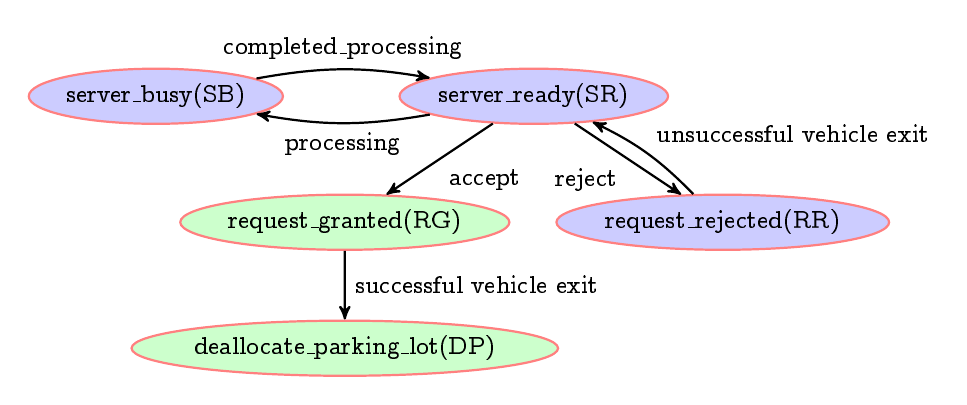
\begin{tikzpicture}[scale=0.4]
			\tikzset{
	%Define standard arrow tip
	>=stealth',
	%Define style for boxes
	punkt/.style={
		rectangle,
		rounded corners,
		draw=black, very thick,
		text width=8.5em,
		minimum height=2em,
		text centered},
	% Define arrow style
	pil/.style={
		->,
		thick,
		shorten <=2pt,
		shorten >=2pt,}
}
\tikzstyle{aldecision} = [diamond, draw, fill=blue!20,
text width=4.5em, text badly centered, node distance=2.5cm, inner sep=0pt]
\tikzstyle{alblock} = [rectangle, draw, fill=blue!20,
text width=5em, text centered, rounded corners, minimum height=4em]
\tikzstyle{line} = [draw, very thick, color=black!50, -latex']
\tikzstyle{allibrary} = [draw, ellipse,fill=red!20, node distance=2.5cm,
minimum height=2em]
		
		\node 	(s1)		at	(0,10) 	[ellipse, thick, draw=red!50,fill=blue!20,inner sep=0pt,minimum height=.70cm, minimum width=1.5cm]{\small server\_ready(SR)};
		
		
		\node 	(s0)		at	(-12,10) 	[ellipse, thick, draw=red!50,fill=blue!20,inner sep=0pt,minimum height=.70cm, minimum width=1.5cm]{\small server\_busy(SB)};
		
		
		\node 	(s2)		at	(-6,6) 	[ellipse, thick, draw=red!50,fill=green!20,inner sep=0pt,minimum height=.70cm, minimum width=1.5cm]{\small request\_granted(RG)};
		
				
		\node 	(s3)		at	(-6,2) 	[ellipse, thick, draw=red!50,fill=green!20,inner sep=0pt,minimum height=.70cm, minimum width=1.5cm]{\small deallocate\_parking\_lot(DP)};
		
				
		\node 	(s4)		at	(6,6) 	[ellipse, thick, draw=red!50,fill=blue!20,inner sep=0pt,minimum height=.70cm, minimum width=1.5cm]{\small request\_rejected(RR)};
		
	
		\draw[->, bend left=10,thick]	(s0)	to	node[auto]{\small completed\_processing}	(s1);
		
		\draw[->, bend left=10, thick]	(s1)	to	node[auto]{\small processing}	(s0);
		
		\draw[->, thick]	(s1)	to	node[auto]{\small accept}	(s2);
		
		\draw[->, thick]	(s1)	to	node[auto,swap]{\small reject}	(s4);
		
		\draw[->, thick]	(s2)	to	node[auto]{\small successful vehicle exit}	(s3);
		
		\draw[->, thick, bend right = 10]	(s4)	to	node[auto,swap]{\small unsuccessful vehicle exit}	(s1);

		
		\end{tikzpicture}
}
\end{figure}
\end{frame}

\begin{frame}{Case Study Parking System: Client behaviour}
\begin{figure}[!ht]
\centering
\scalebox{0.7}{
		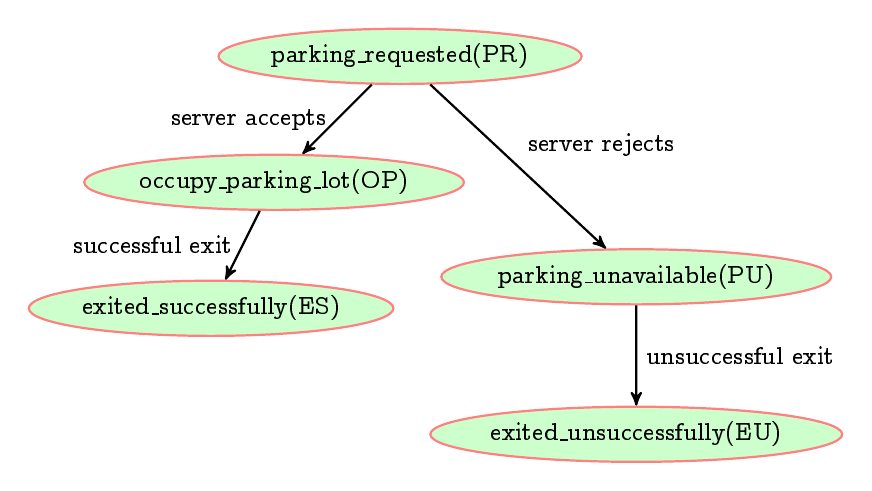
\begin{tikzpicture}[scale=0.4]
			\tikzset{
	%Define standard arrow tip
	>=stealth',
	%Define style for boxes
	punkt/.style={
		rectangle,
		rounded corners,
		draw=black, very thick,
		text width=8.5em,
		minimum height=2em,
		text centered},
	% Define arrow style
	pil/.style={
		->,
		thick,
		shorten <=2pt,
		shorten >=2pt,}
}
\tikzstyle{aldecision} = [diamond, draw, fill=blue!20,
text width=4.5em, text badly centered, node distance=2.5cm, inner sep=0pt]
\tikzstyle{alblock} = [rectangle, draw, fill=blue!20,
text width=5em, text centered, rounded corners, minimum height=4em]
\tikzstyle{line} = [draw, very thick, color=black!50, -latex']
\tikzstyle{allibrary} = [draw, ellipse,fill=red!20, node distance=2.5cm,
minimum height=2em]


		
		
		\node 	(s1)		at	(0,10) 	[ellipse, thick, draw=red!50,fill=green!20,inner sep=0pt,minimum height=.70cm, minimum width=1.5cm]{\small parking\_requested(PR)};
		
		
		
		\node 	(s2)		at	(-4,6) 	[ellipse, thick, draw=red!50,fill=green!20,inner sep=0pt,minimum height=.70cm, minimum width=1.5cm]{\small occupy\_parking\_lot(OP)};
		
				
		\node 	(s3)		at	(-6,2) 	[ellipse, thick, draw=red!50,fill=green!20,inner sep=0pt,minimum height=.70cm, minimum width=1.5cm]{\small exited\_successfully(ES)};
		
				
		\node 	(s4)		at	(7.5,3) 	[ellipse, thick, draw=red!50,fill=green!20,inner sep=0pt,minimum height=.70cm, minimum width=1.5cm]{\small parking\_unavailable(PU)};
		
		\node 	(s5)		at	(7.5,-2) 	[ellipse, thick, draw=red!50,fill=green!20,inner sep=0pt,minimum height=.70cm, minimum width=1.5cm]{\small exited\_unsuccessfully(EU)};

		
		\draw[->, thick]	(s1)	to	node[left]{\small server accepts}	(s2);
		
		\draw[->, thick]	(s1)	to	node[auto]{\small server rejects}	(s4);
		
		\draw[->, thick]	(s2)	to	node[left]{\small successful exit}	(s3);
		
		\draw[->, thick]	(s4)	to	node[auto]{\small unsuccessful exit}	(s5);
		

		
		\end{tikzpicture}
}
\end{figure}
\end{frame}


\begin{frame}\frametitle{Modelling an Unbounded Client-Server (UCS)}
\begin{columns}[T] % align columns
\begin{column}{.5\textwidth}
\begin{figure}
\begin{center}
\scalebox{0.8}{	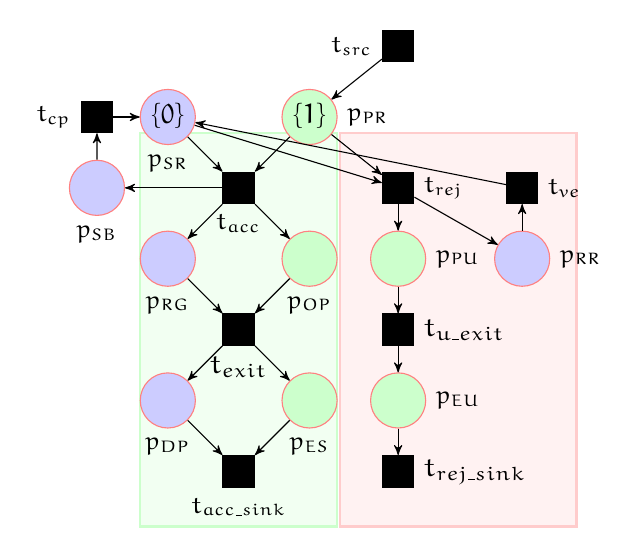
\begin{tikzpicture}[scale=0.45]
				\tikzset{
	%Define standard arrow tip
	>=stealth',
	%Define style for boxes
	punkt/.style={
		rectangle,
		rounded corners,
		draw=black, very thick,
		text width=8.5em,
		minimum height=2em,
		text centered},
	% Define arrow style
	pil/.style={
		->,
		thick,
		shorten <=2pt,
		shorten >=2pt,}
}
\tikzstyle{aldecision} = [diamond, draw, fill=blue!20,
text width=4.5em, text badly centered, node distance=2.5cm, inner sep=0pt]
\tikzstyle{alblock} = [rectangle, draw, fill=blue!20,
text width=5em, text centered, rounded corners, minimum height=4em]
\tikzstyle{line} = [draw, very thick, color=black!50, -latex']
\tikzstyle{allibrary} = [draw, ellipse,fill=red!20, node distance=2.5cm,
minimum height=2em]


%	\begin{center}

		
		\node 	at	(-3,-8) 	[rectangle, thick, draw=green!20, fill=green!5,inner sep=0pt,minimum height=5cm, minimum width=2.5cm] (bga){};
		
		
		\node 	at	(3.2,-8) 	[rectangle, thick, draw=red!20, fill=red!5,inner sep=0pt,minimum height=5cm, minimum width=3cm] (bgr){};
		
		%source transition
		\node[transition,fill=black,minimum height=.4cm,minimum width=.4cm,label=left:{\small $t_{src}$}] (t0) at (1.5,0) {};
		
		%parking requested client place
		\node[place,label=right:{\small $p_{PR}$},draw=red!50,fill=green!20,inner
sep=0pt,minimum height=.40cm, minimum width=.7cm] (p0) at (-1,-2){$\{1\}$} ;	
		
		%server ready place			
		\node[place,label=below:{\small $p_{SR}$},draw=red!50,fill=blue!20,inner
sep=0pt,minimum height=.40cm, minimum width=.7cm] (p1) at (-5,-2){$\{0\}$} ;

%places and transitions for request granted scenarios		
		%accept transition
		\node[transition,fill=black,minimum height=.4cm,minimum width=.4cm,label=below:{\small $t_{acc}$}] (t1) at (-3,-4) {};
		
		%server busy place
		\node[place,label=below:{\small $p_{SB}$},draw=red!50,fill=blue!20,inner
sep=0pt,minimum height=.40cm, minimum width=.7cm] (p7) at (-7,-4){} ;

		%processing complete
		\node[transition,fill=black,minimum height=.4cm,minimum width=.4cm,label=left:{\small $t_{cp}$}] (t6) at (-7,-2) {};
		
		%client place occupy parking lot op
		\node[place,label=below:{\small $p_{OP}$},draw=red!50,fill=green!20,inner
sep=0pt,minimum height=.40cm, minimum width=.7cm] (p2) at (-1,-6){} ;	
		
		%server place request granted rg	
		\node[place,label=below:{\small $p_{RG}$},draw=red!50,fill=blue!20,inner
sep=0pt,minimum height=.40cm, minimum width=.7cm] (p3) at (-5,-6){} ;
		

		%transition exit
		\node[transition,fill=black,minimum height=.4cm,minimum width=.4cm,label=below:{$t_{exit}$}] (t2) at (-3,-8) {};
		
		%client place Exit successfully ES
		\node[place,label=below:{\small $p_{ES}$},draw=red!50,fill=green!20,inner
sep=0pt,minimum height=.40cm, minimum width=.7cm] (p4) at (-1,-10){} ;			

		%server place deallocate parking lot DP
		\node[place,label=below:{\small $p_{DP}$},draw=red!50,fill=blue!20,inner
sep=0pt,minimum height=.40cm, minimum width=.7cm] (p5) at (-5,-10){} ;
		
		%transition accept sink
		\node[transition,fill=black,minimum height=.4cm,minimum width=.4cm,label=below:{\small $t_{acc\_sink}$}] (t3) at (-3,-12) {};
		
%request rejected scenarios		
		
		%reject transition
		\node[transition,fill=black,minimum height=.4cm,minimum width=.4cm,label=right:{\small $t_{rej}$}] (t4) at (1.5,-4) {};


		%client place parking unavailable PU
		\node[place,label=right:{\small $p_{PU}$},draw=red!50,fill=green!20,inner
sep=0pt,minimum height=.40cm, minimum width=.7cm] (p6) at (1.5,-6){} ;

		% transition unsuccessful exit
		\node[transition,fill=black,minimum height=.4cm,minimum width=.4cm,label=right:{$t_{u\_exit}$}] (t5) at (1.5,-8) {};

            \node[place,label=right:{\small $p_{EU}$},draw=red!50,fill=green!20,inner
sep=0pt,minimum height=.40cm, minimum width=.7cm] (peu) at (1.5,-10){} ;


\node[transition,fill=black,minimum height=.4cm,minimum width=.4cm,label=right:{$t_{rej\_sink}$}] (trej) at (1.5,-12) {};

		%server place request rejected RR
		\node[place,label=right:{\small $p_{RR}$},draw=red!50,fill=blue!20,inner
sep=0pt,minimum height=.40cm, minimum width=.7cm] (p8) at (5,-6){} ;


		%transition exit vehicle ev
		\node[transition,fill=black,minimum height=.4cm,minimum width=.4cm,label=right:{\small $t_{ve}$}] (t7) at (5,-4) {};
				
		\draw[->] (t0) -- (p0);
		\draw[->] (p0) -- (t1);
		\draw[->] (p1) -- (t4);
		\draw[->] (t1) -- (p7);
		\draw[->] (p7) -- (t6);		
 	        \draw[->] (t6) -- (p1);
		\draw[->] (p1) -- (t1);
		\draw[->] (t1) -- (p2); 
		\draw[->] (p2) -- (t2);
		\draw[->] (t2) -- (p4);
		\draw[->] (p4) -- (t3);
		\draw[->] (t1) -- (p3);
		\draw[->] (p3) -- (t2);
		\draw[->] (t2) -- (p5);
		\draw[->] (p5) -- (t3);
		\draw[->] (p0) -- (t4);
		\draw[->] (t4) -- (p6);
		\draw[->] (p6) -- (t5);
		\draw[->] (t4) -- (p8);
		\draw[->] (p8) -- (t7);
		\draw[->] (t7) -- (p1);	
  
            \draw[->] (t5) -- (peu);	
            \draw[->] (peu) -- (trej);	

		
	\end{tikzpicture}
%\end{center}
			
%\vspace{-10pt}
		%\caption{Petri net for UPS with $M_0=(0,0,0,0,0)$}
%		\caption{Petri net for APS}  
%		\label{fig:APS}

}
\end{center}
\end{figure}
\end{column}
\hfill
\begin{column}{.5\textwidth}
Finite sets of atomic client propositions $P_c$ and server propositions $P_s$:
\small{
\begin{align*}
  P_c
    &=\{parking\_requested (PR),\\
    &\qquad~occupy\_parking\_lot (OP),\\
    &\qquad~parking\_unavailable (PU),\\ 
    &\qquad~exit\_successfully (ES),\\
    &\qquad~exited\_unsuccessfully (EU)\}\\
  P_s
    &=\{server\_ready (SR),\\
    &\qquad~server\_busy(SB),\\
    &\qquad~request\_granted (RG),\\
    &\qquad~request\_rejected(RR),\\
    &\qquad~deallocate\_parking\_lot (DP)\}
\end{align*}
}
\end{column}%
\end{columns}
\end{frame}

\begin{frame}{}
    \centering    
    \huge{Question: What properties of the system are we interested in?}    
\end{frame}



\begin{frame}{Properties}
\begin{enumerate}

\item When a vehicle requests a parking space, it is always the case that for every vehicle, it eventually exits the system, either successfully after being granted a parking space, or unsuccessfully, when its request is denied.
\pause
\begin{align*}
    &\mathbf{G}_s(\forall x) \Big( parking\_requested(x) \Rightarrow \\
    & \qquad\mathbf{F}_c~ (exit\_successfully(x)~\lor~exit\_unsuccessfully(x)) \Big)
\end{align*}
\pause
\item It is always the case that if the client occupies a parking lot, it will eventually exit the parking lot. \pause
\begin{align*}
    &\mathbf{G}_s(\forall x) \Big(occupy\_parking\_lot(x)\Rightarrow \mathbf{F}_c(exit\_successfully(x))\Big)
\end{align*}     
 %We expect that this property will hold true. 
\end{enumerate}
\end{frame}


\begin{frame}{Properties}
\begin{enumerate}
\setcounter{enumi}{2}
\item There may be clients whose requests are rejected.\pause
\begin{align*}
 &\mathbf{G}_s(\exists x) \big(parking\_requested(x) \land \mathbf{F}_c (exit\_unsuccessfully(x))\big)
\end{align*}
\pause
\item There may be clients who have requested for parking and who wait in the parking unavailable state until they are able to exit the system.\pause
\begin{align*}
&\mathbf{G}_s(\exists x) \bigg( parking\_requested(x)~\land \\
&\mathbf{F}_c \big( parking\_unavailable(x)~\mathbf{U}_c~exit\_unsuccessfully(x)\big)\bigg)
\end{align*}
\end{enumerate}
\end{frame}

	
\begin{frame}
\frametitle{The proposed logic: The Monodic\footnote{Decidable fragment of first-order temporal logics. Hodkinson et al. '00} Logic {\Lstar}}

\subsection{Syntax}
\visible<1->{
The set of \colorbox{green!30}{client formulae} $\Delta$:
\[\Delta ::= p(x)\mid \lnot\alpha \mid \alpha\lor\beta \mid  \alpha \land \beta \mid \mathbf{X}_c \alpha\mid \mathbf{F}_c\alpha \mid \mathbf{G}_c \alpha \mid \alpha ~\mathbf{U}_c~ \beta\]

where $\alpha,\beta \in \Delta$ and $p\in P_c$, the set of atomic client propositions.
}

%\visible<2->{Let $\Phi=\{(\exists x)\alpha,(\forall x)\alpha \mid \alpha \in \Delta\}$.}

\visible<2->{
The set of  \colorbox{green!30}{server formulae} $\Psi$:
\begin{equation}
    \begin{split}    
    \Psi ::= & q \mid \lnot \psi \mid (\exists x)\alpha \mid (\forall x)\alpha \mid\psi_1 \lor \psi_2 \mid \psi_1\land \psi_2 \mid\\ \nonumber
    & \mathbf{X_s} \psi \mid \mathbf{F_s} \psi \mid \mathbf{G_s}\psi \mid \psi_1 ~\mathbf{U_s}~\psi_2
    \end{split}
\end{equation}
where $\psi, \psi_1, \psi_2 \in \Psi$ and $q \in P_s$, the set of atomic server propositions, $\alpha \in \Delta$.
}

\end{frame}




\begin{frame}
\frametitle{The Monodic Logic {\Lstar} (contd)}
%\textcolor{red}{TODO: write this in words instead?}
\[\psi = (\exists x)(\exists y) \bigg(\big(PR(x) \land PR(y)\big)\land \mathbf{F_c}\big(ES(x) \land ES(y)\big)\bigg)\]
\begin{itemize}[<+->]
\item Is $\psi\in$ {\Lstar}?
\item \textcolor{purple}{Answer: No. \textbf{not a well formed formula} in {\Lstar}}% $\psi$ is a non-monodic formula which is \textbf{not a well formed formula} in {\Lstar}.}
%\end{itemize}
%\begin{itemize}    
%\item[] Note: 
%\item[-]  In server formula $\Psi$ every variable is bounded.

%\item[-] In {\Lstar}, the quantifier depth is atmost one. 
%\item[-] Quantifier alternation is not allowed.
\end{itemize}
\end{frame}


\begin{frame}\frametitle{Recall: our model}
\begin{columns}[T] % align columns
\begin{column}{.5\textwidth}
\begin{figure}
\begin{center}
\scalebox{0.8}{	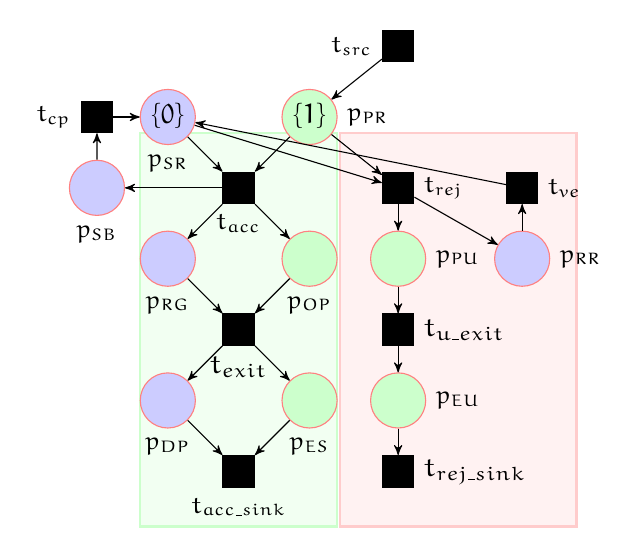
\begin{tikzpicture}[scale=0.45]
				\tikzset{
	%Define standard arrow tip
	>=stealth',
	%Define style for boxes
	punkt/.style={
		rectangle,
		rounded corners,
		draw=black, very thick,
		text width=8.5em,
		minimum height=2em,
		text centered},
	% Define arrow style
	pil/.style={
		->,
		thick,
		shorten <=2pt,
		shorten >=2pt,}
}
\tikzstyle{aldecision} = [diamond, draw, fill=blue!20,
text width=4.5em, text badly centered, node distance=2.5cm, inner sep=0pt]
\tikzstyle{alblock} = [rectangle, draw, fill=blue!20,
text width=5em, text centered, rounded corners, minimum height=4em]
\tikzstyle{line} = [draw, very thick, color=black!50, -latex']
\tikzstyle{allibrary} = [draw, ellipse,fill=red!20, node distance=2.5cm,
minimum height=2em]


%	\begin{center}

		
		\node 	at	(-3,-8) 	[rectangle, thick, draw=green!20, fill=green!5,inner sep=0pt,minimum height=5cm, minimum width=2.5cm] (bga){};
		
		
		\node 	at	(3.2,-8) 	[rectangle, thick, draw=red!20, fill=red!5,inner sep=0pt,minimum height=5cm, minimum width=3cm] (bgr){};
		
		%source transition
		\node[transition,fill=black,minimum height=.4cm,minimum width=.4cm,label=left:{\small $t_{src}$}] (t0) at (1.5,0) {};
		
		%parking requested client place
		\node[place,label=right:{\small $p_{PR}$},draw=red!50,fill=green!20,inner
sep=0pt,minimum height=.40cm, minimum width=.7cm] (p0) at (-1,-2){$\{1\}$} ;	
		
		%server ready place			
		\node[place,label=below:{\small $p_{SR}$},draw=red!50,fill=blue!20,inner
sep=0pt,minimum height=.40cm, minimum width=.7cm] (p1) at (-5,-2){$\{0\}$} ;

%places and transitions for request granted scenarios		
		%accept transition
		\node[transition,fill=black,minimum height=.4cm,minimum width=.4cm,label=below:{\small $t_{acc}$}] (t1) at (-3,-4) {};
		
		%server busy place
		\node[place,label=below:{\small $p_{SB}$},draw=red!50,fill=blue!20,inner
sep=0pt,minimum height=.40cm, minimum width=.7cm] (p7) at (-7,-4){} ;

		%processing complete
		\node[transition,fill=black,minimum height=.4cm,minimum width=.4cm,label=left:{\small $t_{cp}$}] (t6) at (-7,-2) {};
		
		%client place occupy parking lot op
		\node[place,label=below:{\small $p_{OP}$},draw=red!50,fill=green!20,inner
sep=0pt,minimum height=.40cm, minimum width=.7cm] (p2) at (-1,-6){} ;	
		
		%server place request granted rg	
		\node[place,label=below:{\small $p_{RG}$},draw=red!50,fill=blue!20,inner
sep=0pt,minimum height=.40cm, minimum width=.7cm] (p3) at (-5,-6){} ;
		

		%transition exit
		\node[transition,fill=black,minimum height=.4cm,minimum width=.4cm,label=below:{$t_{exit}$}] (t2) at (-3,-8) {};
		
		%client place Exit successfully ES
		\node[place,label=below:{\small $p_{ES}$},draw=red!50,fill=green!20,inner
sep=0pt,minimum height=.40cm, minimum width=.7cm] (p4) at (-1,-10){} ;			

		%server place deallocate parking lot DP
		\node[place,label=below:{\small $p_{DP}$},draw=red!50,fill=blue!20,inner
sep=0pt,minimum height=.40cm, minimum width=.7cm] (p5) at (-5,-10){} ;
		
		%transition accept sink
		\node[transition,fill=black,minimum height=.4cm,minimum width=.4cm,label=below:{\small $t_{acc\_sink}$}] (t3) at (-3,-12) {};
		
%request rejected scenarios		
		
		%reject transition
		\node[transition,fill=black,minimum height=.4cm,minimum width=.4cm,label=right:{\small $t_{rej}$}] (t4) at (1.5,-4) {};


		%client place parking unavailable PU
		\node[place,label=right:{\small $p_{PU}$},draw=red!50,fill=green!20,inner
sep=0pt,minimum height=.40cm, minimum width=.7cm] (p6) at (1.5,-6){} ;

		% transition unsuccessful exit
		\node[transition,fill=black,minimum height=.4cm,minimum width=.4cm,label=right:{$t_{u\_exit}$}] (t5) at (1.5,-8) {};

            \node[place,label=right:{\small $p_{EU}$},draw=red!50,fill=green!20,inner
sep=0pt,minimum height=.40cm, minimum width=.7cm] (peu) at (1.5,-10){} ;


\node[transition,fill=black,minimum height=.4cm,minimum width=.4cm,label=right:{$t_{rej\_sink}$}] (trej) at (1.5,-12) {};

		%server place request rejected RR
		\node[place,label=right:{\small $p_{RR}$},draw=red!50,fill=blue!20,inner
sep=0pt,minimum height=.40cm, minimum width=.7cm] (p8) at (5,-6){} ;


		%transition exit vehicle ev
		\node[transition,fill=black,minimum height=.4cm,minimum width=.4cm,label=right:{\small $t_{ve}$}] (t7) at (5,-4) {};
				
		\draw[->] (t0) -- (p0);
		\draw[->] (p0) -- (t1);
		\draw[->] (p1) -- (t4);
		\draw[->] (t1) -- (p7);
		\draw[->] (p7) -- (t6);		
 	        \draw[->] (t6) -- (p1);
		\draw[->] (p1) -- (t1);
		\draw[->] (t1) -- (p2); 
		\draw[->] (p2) -- (t2);
		\draw[->] (t2) -- (p4);
		\draw[->] (p4) -- (t3);
		\draw[->] (t1) -- (p3);
		\draw[->] (p3) -- (t2);
		\draw[->] (t2) -- (p5);
		\draw[->] (p5) -- (t3);
		\draw[->] (p0) -- (t4);
		\draw[->] (t4) -- (p6);
		\draw[->] (p6) -- (t5);
		\draw[->] (t4) -- (p8);
		\draw[->] (p8) -- (t7);
		\draw[->] (t7) -- (p1);	
  
            \draw[->] (t5) -- (peu);	
            \draw[->] (peu) -- (trej);	

		
	\end{tikzpicture}
%\end{center}
			
%\vspace{-10pt}
		%\caption{Petri net for UPS with $M_0=(0,0,0,0,0)$}
%		\caption{Petri net for APS}  
%		\label{fig:APS}

}
\end{center}
\end{figure}
\end{column}
\hfill
\begin{column}{.5\textwidth}
Atomic client propositions $P_c$ and server propositions $P_s$:
\small{
\begin{align*}
  P_c
    &=\{parking\_requested (PR),\\
    &\qquad~occupy\_parking\_lot (OP),\\
    &\qquad~parking\_unavailable (PU),\\ 
    &\qquad~exit\_successfully (ES),\\
    &\qquad~exited\_unsuccessfully (EU)\}\\
  P_s
    &=\{server\_ready (SR),\\
    &\qquad~server\_busy(SB),\\
    &\qquad~request\_granted (RG),\\
    &\qquad~request\_rejected(RR),\\
    &\qquad~deallocate\_parking\_lot (DP)\}
\end{align*}
}
\end{column}%
\end{columns}
\end{frame}


\begin{frame}{Snapshots of the system + live windows}
    

\begin{ganttchart}[
vgrid,hgrid,
progress label text=\relax,
x unit=10mm,
title height=1,
foobar top shift=.15,
foobar height=.70
]{0}{2}
\visible<1>{\textganttbar{Client 1}{$p_{PR}$}{0}{0} }
\visible<2>{\textganttbar{Client 1}{$p_{PR}$}{0}{0}  \textganttbar{}{$p_{OP}$}{1}{1}}
\visible<3>{ 
 \textganttbar{Client 1}{$p_{PR}$}{0}{0}  \textganttbar{}{$p_{OP}$}{1}{1} \textganttbar{}{$p_{OP}$}{2}{2}\\ 
\textganttbar{Client 2}{$p_{PR}$}{2}{2}
}



\begin{scope}[yshift=0.33cm]
\draw[->] (0,0) -- (3.7,0);
\draw ([yshift=-3pt]0,0) -- ++([yshift=6pt]0,0) node[xshift=45pt, yshift=15pt, above] {time instance $\rightarrow$};    
\draw ([yshift=-3pt]1,0) -- ++([yshift=6pt]0,0) node[xshift=-10pt, above] {$0$};
\visible<2->{
\draw ([yshift=-3pt]2,0) -- ++([yshift=6pt]0,0) node[xshift=-10pt, above] {$1$};}
\visible<3->{\draw ([yshift=-3pt]3,0) -- ++([yshift=6pt]0,0) node[xshift=-10pt, above] {$2$};}
\end{scope}
\end{ganttchart}         
\end{frame}





\begin{frame}{Snapshots of the system + live windows (contd)}
\begin{columns}[T] % align columns
\begin{column}{.5\textwidth}
\begin{figure}
\begin{center}
\scalebox{0.8}{\begin{ganttchart}[
vgrid,hgrid,
%inline,
progress label text=\relax,
x unit=10mm,
% title top shift=0,
title height=1,
foobar top shift=.15,
foobar height=.70
]{0}{5}
%\gantttitlelist{0,...,5}{1}\\
 \textganttbar{Client 1}{$p_{PR}$}{0}{0}  \textganttbar{}{$p_{OP}$}{1}{1} \textganttbar{}{$p_{ES}$}{2}{2} \\
  \textganttbar{Client 2}{$p_{PR}$}{1}{1}  \textganttbar{}{$p_{PU}$}{2}{2}  \textganttbar{}{$p_{EU}$}{3}{3}\\
   \textganttbar{Client 3}{$p_{PR}$}{3}{3} \textganttbar{}{$p_{PR}$}{4}{4}\textganttbar{}{$p_{PR}$}{5}{5}\\
   \textganttbar{Client 4}{$p_{PR}$}{4}{4} \textganttbar{}{$p_{PR}$}{5}{5}
   \begin{scope}[yshift=0.33cm]
    \draw[->] (0,0) -- (6.5,0);
    
    \draw ([yshift=-3pt]0,0) -- ++([yshift=6pt]0,0) node[xshift=45pt, yshift=15pt, above] {time instance $\rightarrow$};
    
    \draw ([yshift=-3pt]1,0) -- ++([yshift=6pt]0,0) node[xshift=-10pt, above] {$0$};
    \draw ([yshift=-3pt]2,0) -- ++([yshift=6pt]0,0) node[xshift=-10pt, above] {$1$};
    \draw ([yshift=-3pt]3,0) -- ++([yshift=6pt]0,0) node[xshift=-10pt, above] {$2$};
    \draw ([yshift=-3pt]4,0) -- ++([yshift=6pt]0,0) node[xshift=-10pt, above] {$3$};
    \draw ([yshift=-3pt]5,0) -- ++([yshift=6pt]0,0) node[xshift=-10pt, above] {$4$};
    \draw ([yshift=-3pt]6,0) -- ++([yshift=6pt]0,0) node[xshift=-10pt, above] {$\cdots$};
    %\draw ([yshift=-3pt]7,0) -- ++([yshift=6pt]0,0) node[xshift=-10pt, above] {$\cdots$};
\end{scope}
 \end{ganttchart}}
\end{center}
\end{figure}
\end{column}%
\hfill%
\begin{column}{.5\textwidth}
\begin{itemize}
\item $4$ distinguishable clients, with overlapping \emph{live windows}, with the bound $5$.
\item client $1$ is at $p_{PR}$ at instance $0$. i.e, $PR(x)$ is satisfied in client $1$ at instance $0$.
\item For client $1$, the \emph{left boundary} is at instance $0$ and its \emph{right boundary} is at instance $2$.
\end{itemize}
\end{column}%
\end{columns}
\end{frame}




\begin{frame}{Formally speaking...}
\begin{itemize}
\item Let $CN$ be a \colorbox{green!30}{countable set of client names}. \pause
\item Let $CS = (Q,\Sigma,\delta,I,F)$ be a \colorbox{green!30}{finite state machine describing the client behaviour}. \pause
\item Let $L:Q \to 2^{P_c}$ be the labelling function of each client state  $q \in Q$ in terms of a \colorbox{green!30}{subset of propositions $P_c$ true in that state}. \pause

\item Let $\mathfrak{Z}:CN \times \mathbb{N}_0 \to Q$ be a partial mapping describing the local state of each client $a \in CN$ at an instance $i \in \mathbb{N}_0$. \pause
\item[-]For instance, $\mathfrak{Z}(a,i)\in q$, means that the \colorbox{green!30}{local state of each client $a$ at instance $i$ is state $q$}, where $q \in Q$.
\end{itemize}
\end{frame}

\begin{frame}{Formally speaking...}
A model is a triple $M=(\nu,V,\xi)$ where
\begin{itemize}
\item $\nu$ gives the \colorbox{green!30}{local behaviour of the server} as follows:

$\nu=\nu_0\nu_1\nu_2\ldots$, where for all $0 \le i$, $\nu_i \subseteq P_s$ \pause

\item $V$ gives the \colorbox{green!30}{set of live agents (clients) at each instance}. 

$V=V_0V_1V_2\ldots$, where for all $0 \le i$, $V_i$ is a finite subset of $CN$, gives the set of live agents at the $i$th instance.

For every $0\le i$, $V_i$ and $V_{i+1}$ satisfy  the following properties:
\begin{enumerate}
\item if $V_i \subseteq V_{i+1}$ then for every $a \in V_{i+1}-V_i$ such that $\mathfrak{Z}(a,i+1)\in I$.
\item if $V_{i+1}\subseteq V_i$ then for every $a \in V_i-V_{i+1}$ such that $\mathfrak{Z}(a,i)\in F$.
\end{enumerate} \pause

\item $\xi=\xi_0\xi_1\xi_2\cdots$, where for all $0 \le i$, $\xi_i:V_i\to 2^{P_c}$ gives \colorbox{green!30}{the properties satisfied by each live agent at $i$th instance.}
\item[]Also, $L(\mathfrak{Z}(a,i))=\xi_i(a)$. %Alternatively, $\xi_i$ can be given as $\xi_i:V_i\times P_c \to\{\top,\bot\}$. %, an equivalent form.
\end{itemize}
\end{frame}


    
\begin{frame}{Semantics}
\visible<1->{
$M,i \models (\exists x)\alpha$ iff $\exists a\in CN$, $a \in V_i$ and $M,[x\mapsto a],i\models_x \alpha$. 
}

\visible<2->{

$M,i \models^{k} (\exists x)\alpha$ iff $\exists a\in CN$, $a \in V_i$ and $M,[x\mapsto a],i\models^{k}_x \alpha$.
}

\begin{columns}[T] % align columns
\begin{column}{.4\textwidth}
\visible<3->{
\begin{figure}
\begin{center}
\scalebox{0.8}{\begin{ganttchart}[
vgrid,hgrid,
%inline,
progress label text=\relax,
x unit=10mm,
% title top shift=0,
title height=1,
foobar top shift=.15,
foobar height=.70
]{0}{2}
%\gantttitlelist{0,...,5}{1}\\
 \textganttbar{Client 1}{$p_{PR}$}{0}{0}  \textganttbar{}{$p_{OP}$}{1}{1} \textganttbar{}{$p_{OP}$}{2}{2} \\
  \textganttbar{Client 2}{$p_{PR}$}{1}{1}  \textganttbar{}{$p_{PU}$}{2}{2}%  \textganttbar{}{$pc_2$}{3}{3}\\
  % \textganttbar{Client 3}{$pc_1$}{3}{3} \textganttbar{}{$pc_1$}{4}{4}\textganttbar{}{$pc_1$}{5}{5}\\
%   \textganttbar{Client 4}{$pc_1$}{4}{4} \textganttbar{}{$pc_1$}{5}{5}
      \begin{scope}[yshift=0.33cm]
    \draw[-] (0,0) -- (3,0);
    
    %\draw ([yshift=-3pt]0,0) -- ++([yshift=6pt]0,0) node[xshift=-10pt, above] {};
    
    \draw ([yshift=-3pt]0,0) -- ++([yshift=6pt]0,0) node[xshift=45pt, yshift=15pt, above] {time instance $\rightarrow$};

    \draw ([yshift=-3pt]1,0) -- ++([yshift=6pt]0,0) node[xshift=-10pt, above] {$0$};
    \draw ([yshift=-3pt]2,0) -- ++([yshift=6pt]0,0) node[xshift=-10pt, above] {$1$};
    \draw ([yshift=-3pt]3,0) -- ++([yshift=6pt]0,0) node[xshift=-10pt, above] {$2$};
    %\draw ([yshift=-3pt]4,0) -- ++([yshift=6pt]0,0) node[xshift=-10pt, above] {$3$};
   % \draw ([yshift=-3pt]6.5,0) -- ++([yshift=6pt]0,0) node[xshift=-10pt, above] {$\cdots$};
\end{scope}
 \end{ganttchart}}
\end{center}
\end{figure}
}
\end{column}%
\hfill%
\begin{column}{.6\textwidth}
\visible<4->{
\begin{itemize}
\item[] 
Given $\alpha=OP(x) \lor PR(x)$ and  $CN=\{1,2\}$. 
\end{itemize}
}
\visible<5->{
\begin{itemize}
\item $M,0 \models^{k} (\exists x)(OP(x) \lor PR(x))$. 
\item $M,1 \models^{k} (\exists x)(OP(x) \lor PR(x))$.
\item $M,2 \models^{k} (\exists x)(OP(x) \lor PR(x))$.
\end{itemize}
}
\end{column}%
\end{columns}
\end{frame}



\begin{frame}{Bounded Semantics}
$M,i \models^{k} (\forall x)\alpha$ iff $\forall a\in CN$, if $a \in V_i$ then $M,[x\mapsto a],i\models^{k}_x \alpha$
\begin{columns}[T]
\begin{column}{.4\textwidth}
\begin{figure}
\begin{center}
\scalebox{0.8}{\begin{ganttchart}[
vgrid,hgrid,
%inline,
progress label text=\relax,
x unit=10mm,
% title top shift=0,
title height=1,
foobar top shift=.15,
foobar height=.70
]{0}{2}
%\gantttitlelist{0,...,5}{1}\\
 \textganttbar{Client 1}{$p_{PR}$}{0}{0}  \textganttbar{}{$p_{OP}$}{1}{1} \textganttbar{}{$p_{OP}$}{2}{2} \\
  \textganttbar{Client 2}{$p_{PR}$}{1}{1}  \textganttbar{}{$p_{PU}$}{2}{2}%  \textganttbar{}{$pc_2$}{3}{3}\\
  % \textganttbar{Client 3}{$pc_1$}{3}{3} \textganttbar{}{$pc_1$}{4}{4}\textganttbar{}{$pc_1$}{5}{5}\\
%   \textganttbar{Client 4}{$pc_1$}{4}{4} \textganttbar{}{$pc_1$}{5}{5}
      \begin{scope}[yshift=0.33cm]
    \draw[-] (0,0) -- (3,0);
    
    %\draw ([yshift=-3pt]0,0) -- ++([yshift=6pt]0,0) node[xshift=-10pt, above] {};
    
    \draw ([yshift=-3pt]0,0) -- ++([yshift=6pt]0,0) node[xshift=45pt, yshift=15pt, above] {time instance $\rightarrow$};

    \draw ([yshift=-3pt]1,0) -- ++([yshift=6pt]0,0) node[xshift=-10pt, above] {$0$};
    \draw ([yshift=-3pt]2,0) -- ++([yshift=6pt]0,0) node[xshift=-10pt, above] {$1$};
    \draw ([yshift=-3pt]3,0) -- ++([yshift=6pt]0,0) node[xshift=-10pt, above] {$2$};
    %\draw ([yshift=-3pt]4,0) -- ++([yshift=6pt]0,0) node[xshift=-10pt, above] {$3$};
   % \draw ([yshift=-3pt]6.5,0) -- ++([yshift=6pt]0,0) node[xshift=-10pt, above] {$\cdots$};
\end{scope}
 \end{ganttchart}}
\end{center}
\end{figure}
\end{column}
\hfill
\begin{column}{.6\textwidth}
\begin{itemize}
\item[] 
Given $\alpha=ES(x)$ and  $CN=\{1,2\}$.
\item $M,0 \not\models^{k} (\exists x)(ES(x))$.
\item $M,1 \not\models^{k} (\exists x)(ES(x))$.
\item $M,2 \not\models^{k} (\exists x)(ES(x))$.
\end{itemize}
\end{column}
\end{columns}
\end{frame}


\begin{frame}{Bounded Semantics}
$M,i\models^{k} \mathbf{F_s}\psi$ iff $\exists j: i \le j \le k$ , $M,j\models^{k} \psi$.

Given $\psi= (\exists x)ES(x)$. 
\begin{columns}[T]
\begin{column}{.5\textwidth}
\begin{figure}
\begin{center}
\scalebox{0.8}{\input{figures/live_windows_overlap_line_3}}
\end{center}
\caption{Snapshot with 4 clients}
\label{fig:4clients}
\end{figure}
\end{column}
\hfill
\begin{column}{.5\textwidth}
\begin{figure}
\begin{center}
\scalebox{0.8}{\begin{ganttchart}[
vgrid,hgrid,
%inline,
progress label text=\relax,
x unit=10mm,
% title top shift=0,
title height=1,
foobar top shift=.15,
foobar height=.70
]{0}{2}
%\gantttitlelist{0,...,5}{1}\\
 \textganttbar{Client 1}{$p_{PR}$}{0}{0}  \textganttbar{}{$p_{OP}$}{1}{1} \textganttbar{}{$p_{OP}$}{2}{2} \\
  \textganttbar{Client 2}{$p_{PR}$}{1}{1}  \textganttbar{}{$p_{PU}$}{2}{2}%  \textganttbar{}{$pc_2$}{3}{3}\\
  % \textganttbar{Client 3}{$pc_1$}{3}{3} \textganttbar{}{$pc_1$}{4}{4}\textganttbar{}{$pc_1$}{5}{5}\\
%   \textganttbar{Client 4}{$pc_1$}{4}{4} \textganttbar{}{$pc_1$}{5}{5}
      \begin{scope}[yshift=0.33cm]
    \draw[-] (0,0) -- (3,0);
    
    %\draw ([yshift=-3pt]0,0) -- ++([yshift=6pt]0,0) node[xshift=-10pt, above] {};
    
    \draw ([yshift=-3pt]0,0) -- ++([yshift=6pt]0,0) node[xshift=45pt, yshift=15pt, above] {time instance $\rightarrow$};

    \draw ([yshift=-3pt]1,0) -- ++([yshift=6pt]0,0) node[xshift=-10pt, above] {$0$};
    \draw ([yshift=-3pt]2,0) -- ++([yshift=6pt]0,0) node[xshift=-10pt, above] {$1$};
    \draw ([yshift=-3pt]3,0) -- ++([yshift=6pt]0,0) node[xshift=-10pt, above] {$2$};
    %\draw ([yshift=-3pt]4,0) -- ++([yshift=6pt]0,0) node[xshift=-10pt, above] {$3$};
   % \draw ([yshift=-3pt]6.5,0) -- ++([yshift=6pt]0,0) node[xshift=-10pt, above] {$\cdots$};
\end{scope}
 \end{ganttchart}}
\end{center}
\caption{Snapshot with 2 clients}
\label{fig:2clients}
\end{figure}
\end{column}
\end{columns} \pause
As shown above $M,5\models^{k} \mathbf{F_s}(\exists x)ES(x)$.
\end{frame}



\begin{frame}
	\frametitle{Takeaway}	
	\begin{itemize}
		\item Proposed the logic {\Lstar} for client-server specifications.
		\item Modeled the running example using nets.
            \item Detailed Semantics and encoding are in our paper!
            \item Currently working on building a model checker to verify {\Lstar} properties.
            
	\end{itemize}
\begin{center}Thank you for your attention\end{center}
\end{frame}




\appendix
\begin{frame}
\centering
\huge{Appendix}    
\end{frame}


\begin{frame}{Bounded Semantics}
$M,[x\mapsto a],i\models^{k}_x \mathbf{F}_c\alpha$ iff\\
$\exists j: i \le j \le k$, $a\in V_j$ and $M,[x\mapsto a],j\models^{k}_x \alpha$.


\begin{columns}[T]
\begin{column}{.5\textwidth}
\begin{figure}
\begin{center}
\scalebox{0.8}{\input{figures/live_windows_overlap_line_3}}
\end{center}
\caption{Snapshot with 4 clients}
\label{fig:4clients}
\end{figure}
\end{column}
\hfill
\begin{column}{.5\textwidth}
\begin{figure}
\begin{center}
\scalebox{0.8}{\begin{ganttchart}[
vgrid,hgrid,
%inline,
progress label text=\relax,
x unit=10mm,
% title top shift=0,
title height=1,
foobar top shift=.15,
foobar height=.70
]{0}{2}
%\gantttitlelist{0,...,5}{1}\\
 \textganttbar{Client 1}{$p_{PR}$}{0}{0}  \textganttbar{}{$p_{OP}$}{1}{1} \textganttbar{}{$p_{OP}$}{2}{2} \\
  \textganttbar{Client 2}{$p_{PR}$}{1}{1}  \textganttbar{}{$p_{PU}$}{2}{2}%  \textganttbar{}{$pc_2$}{3}{3}\\
  % \textganttbar{Client 3}{$pc_1$}{3}{3} \textganttbar{}{$pc_1$}{4}{4}\textganttbar{}{$pc_1$}{5}{5}\\
%   \textganttbar{Client 4}{$pc_1$}{4}{4} \textganttbar{}{$pc_1$}{5}{5}
      \begin{scope}[yshift=0.33cm]
    \draw[-] (0,0) -- (3,0);
    
    %\draw ([yshift=-3pt]0,0) -- ++([yshift=6pt]0,0) node[xshift=-10pt, above] {};
    
    \draw ([yshift=-3pt]0,0) -- ++([yshift=6pt]0,0) node[xshift=45pt, yshift=15pt, above] {time instance $\rightarrow$};

    \draw ([yshift=-3pt]1,0) -- ++([yshift=6pt]0,0) node[xshift=-10pt, above] {$0$};
    \draw ([yshift=-3pt]2,0) -- ++([yshift=6pt]0,0) node[xshift=-10pt, above] {$1$};
    \draw ([yshift=-3pt]3,0) -- ++([yshift=6pt]0,0) node[xshift=-10pt, above] {$2$};
    %\draw ([yshift=-3pt]4,0) -- ++([yshift=6pt]0,0) node[xshift=-10pt, above] {$3$};
   % \draw ([yshift=-3pt]6.5,0) -- ++([yshift=6pt]0,0) node[xshift=-10pt, above] {$\cdots$};
\end{scope}
 \end{ganttchart}}
\end{center}
\caption{Snapshot with 2 clients}
\label{fig:2clients}
\end{figure}
\end{column}
\end{columns}
Given $\alpha=PR(x)$. The above formula is satisfiable for all clients in both figures.
\end{frame}



\begin{comment}
\begin{frame}{Some \emph{more} observations about {\Lstar}}
We can write monodic formulas using predicates in $P_c$ as follows:
 \[\psi_1 = (\forall x) \Big( \mathbf{G}_c \big(new(x) \Rightarrow \mathbf{F}_c~ exit(x) \big)\Big)\]
 
 \begin{itemize}

\item In $\psi_1$, there is one free variable $x$ in the scope of $\mathbf{G}_c$ as well as $\mathbf{F}_c$. 
 \[\psi_2 = \mathbf{G_s} (\forall x) \Big( new(x) \Rightarrow \mathbf{F}_c~ exit(x)\Big)\]
\item Whereas, in $\psi_2$, there is \textbf{no free variable} in the scope of $\mathbf{G_s}$.


 \[\psi_3 = \mathbf{G_s} (\exists x) new(x) \land \mathbf{F_s}(\exists y) new(y)\]

\item In $\psi_3$, there are \textbf{no free variables} either in the scope of $\mathbf{G_s}$ or $\mathbf{F_s}$. 

\end{itemize}
\end{frame}

\begin{frame}{}
    \centering
    \visible<1>{\huge{Question: What is a suitable formal model for the system?}}
    \visible<2>{\sout{\huge{Question: What is a suitable}} \\\sout{\huge{formal model for the system?}}
    \small{\textcolor{purple}{Question: What are the requirements of the formal model?}}}
\end{frame}


\begin{frame}{Requirements in the formal model}
\begin{itemize}
    \item 
\end{itemize}
\end{frame}


\begin{frame}{Recall: Petri Nets}
\begin{columns}[T] % align columns
\begin{column}{.6\textwidth}
\begin{itemize}
    \item Petri Nets are a useful formalism to model \colorbox{green!30}{concurrent systems}        
    \item Directed bipartite graph with two types of nodes- places and transitions
    \item A Petri Net structure is a tuple $N=(P,T,F,W)$
    \begin{itemize}
        \item a finite set of \colorbox{green!30}{places P}
        \item a finite set of \colorbox{green!30}{transitions T}
        \item $F \subseteq (P \times T) \cup (T \times P)$ is the \colorbox{green!30}{flow relation}
        \item $W:F\rightarrow \aleph_0$ is a \colorbox{green!30}{weight function}, where $\aleph_0$ is the set of non-negative integers. 
    \end{itemize}
\item  \colorbox{green!30}{Marking} $M : P \rightarrow \aleph_0$ (distribution of tokens in places).
\end{itemize}
\end{column}
\begin{column}{.4\textwidth}
\begin{figure}[!ht]
\centering
\scalebox{0.7}{\input{figures/fig_simplenet.tex}}
\label{fig:samplenet}
\end{figure}
\end{column}
\end{columns}
\end{frame}


\begin{frame}{Recall: Petri Nets (continued)}
\begin{columns}[T] % align columns
\begin{column}{.6\textwidth}

\begin{itemize}
\item Here, pre-places of transition $t_0$: $p_0$ and $p_1$.
\item A transition $t$ is \colorbox{green!30}{enabled} at marking $M$, if for each pre-place $p$ of $t$ we have \colorbox{green!30}{$M(p) \geq W(p,t)$}.
%\item \textcolor{purple}{Is transition $t_0$ enabled?}
\item An enabled transition may/may not fire
\item A new marking is obtained when an \colorbox{green!30}{enabled transition 
is fired}\begin{itemize}
    \item From each pre-place $p$ of $t$, \colorbox{green!30}{remove $W(p,t)$} tokens
    \item And \colorbox{green!30}{add $W(t,p)$}  tokens to each post-place $p$ of $t$
\end{itemize} 
\end{itemize}
\end{column}
\begin{column}{.4\textwidth}
\begin{figure}[!ht]
\centering
\scalebox{0.7}{\input{figures/fig_simplenet.tex}}
\label{fig:samplenet}
\end{figure}



\end{column}
\end{columns}
\end{frame}



%demonstrating firing of tokens
\begin{frame}{Firing of transition $t_0$}
\begin{columns}[T] % align columns
\begin{column}{.4\textwidth}
\begin{figure}[!ht]
\centering
\scalebox{0.7}{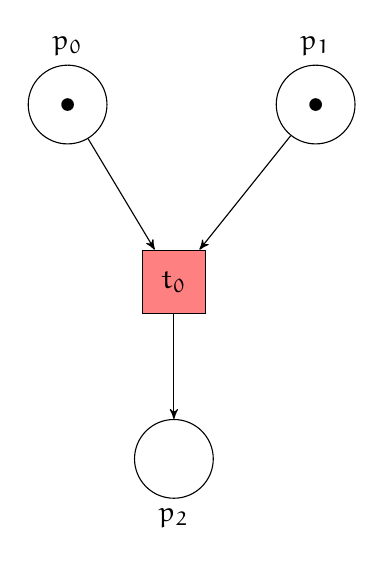
\begin{tikzpicture}[scale=0.45]
				\tikzset{
	%Define standard arrow tip
	>=stealth',
	%Define style for boxes
	punkt/.style={
		rectangle,
		rounded corners,
		draw=black, very thick,
		text width=8.5em,
		minimum height=2em,
		text centered},
	% Define arrow style
	pil/.style={
		->,
		thick,
		shorten <=2pt,
		shorten >=2pt,}
}
\tikzstyle{aldecision} = [diamond, draw, fill=blue!20,
text width=4.5em, text badly centered, node distance=2.5cm, inner sep=0pt]
\tikzstyle{alblock} = [rectangle, draw, fill=blue!20,
text width=5em, text centered, rounded corners, minimum height=4em]
\tikzstyle{line} = [draw, very thick, color=black!50, -latex']
\tikzstyle{allibrary} = [draw, ellipse,fill=red!20, node distance=2.5cm,
minimum height=2em]

\node[place,label=above:$p_0$,inner
sep=0pt,minimum height=1cm, minimum width=1cm, tokens=1] (p0) at (0,0){} ;
\node[place,label=above:$p_1$,inner
sep=0pt,minimum height=1cm, minimum width=1cm, tokens=1] (p1) at (7,0){} ;
\node[place,label=below:$p_2$,inner
sep=0pt,minimum height=1cm, minimum width=1cm] (p2) at (3,-10){} ;
\node[transition,minimum height=0.8cm,minimum width=0.8cm, fill=red!50] (t1) at (3,-5) {$t_0$};
\path[->] (p0) edge(t1);
\path[->] (p1) edge(t1);
\path[->] (t1) edge(p2);
\end{tikzpicture}}
\label{fig:firing_net_lhs}
\end{figure}
\begin{center}
$
\begin{bmatrix}
\colorbox{green!30}{1}\\
\colorbox{green!30}{1}\\
0\\
\end{bmatrix}
$
\end{center}
\end{column}
\begin{column}{0.2\textwidth}
\begin{center}
    $\xrightarrow{t_0}$
\end{center}


\end{column}
\begin{column}{.4\textwidth}
\begin{figure}[!ht]
\centering
\scalebox{0.7}{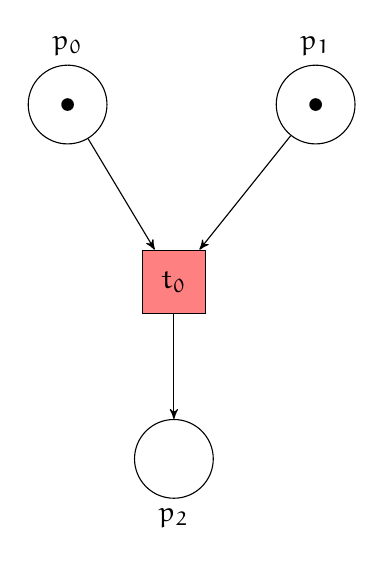
\begin{tikzpicture}[scale=0.45]
				\tikzset{
	%Define standard arrow tip
	>=stealth',
	%Define style for boxes
	punkt/.style={
		rectangle,
		rounded corners,
		draw=black, very thick,
		text width=8.5em,
		minimum height=2em,
		text centered},
	% Define arrow style
	pil/.style={
		->,
		thick,
		shorten <=2pt,
		shorten >=2pt,}
}
\tikzstyle{aldecision} = [diamond, draw, fill=blue!20,
text width=4.5em, text badly centered, node distance=2.5cm, inner sep=0pt]
\tikzstyle{alblock} = [rectangle, draw, fill=blue!20,
text width=5em, text centered, rounded corners, minimum height=4em]
\tikzstyle{line} = [draw, very thick, color=black!50, -latex']
\tikzstyle{allibrary} = [draw, ellipse,fill=red!20, node distance=2.5cm,
minimum height=2em]

\node[place,label=above:$p_0$,inner
sep=0pt,minimum height=1cm, minimum width=1cm, tokens=1] (p0) at (0,0){} ;
\node[place,label=above:$p_1$,inner
sep=0pt,minimum height=1cm, minimum width=1cm, tokens=1] (p1) at (7,0){} ;
\node[place,label=below:$p_2$,inner
sep=0pt,minimum height=1cm, minimum width=1cm] (p2) at (3,-10){} ;
\node[transition,minimum height=0.8cm,minimum width=0.8cm, fill=red!50] (t1) at (3,-5) {$t_0$};
\path[->] (p0) edge(t1);
\path[->] (p1) edge(t1);
\path[->] (t1) edge(p2);
\end{tikzpicture}}

\label{fig:samplenet_rhs}
\end{figure}
\begin{center}
$
\begin{bmatrix}
0\\
0\\
\colorbox{green!30}{1}\\
\end{bmatrix}
$
\end{center}
\end{column}
\end{columns}
\end{frame}


\begin{frame}{Introducing $\nu$-nets}
\begin{itemize}
    \item $S$ is a set of service names, with function $arity: S\to \mathbb{N}$
\item The set of synchronizing labels \emph{Sync}=$\{s(i) \vert s \in S, 1 \leq i \leq arity(s)\}$.
\begin{itemize}
    \item If $arity=2$, we write $s?$ and $s!$ instead of $s(1), s(2)$ respectively, to denote the offer and request of a service.
    \item $A$ is the set of labels with arity $1$. We identify $s\in A$ by $s(1)$. 
\end{itemize}
\item Here, we utilize only labels of arity $1$.
\end{itemize}   
\end{frame}


\begin{frame}{Parking system as a $\nu$-net}
\begin{columns}
\begin{column}{.6\textwidth}
\begin{itemize}
    \item Distinguishable tokens taken from an arbitrary infinite set Id
    \item A finite set of variables $Var$
    \item Arcs are labeled by $v \in Var$.
    \item Create fresh names using a special variable $\nu \in Var$ that appears only in post condition arcs
\end{itemize} 
\end{column}
\begin{column}{.4\textwidth}
\begin{figure}[!ht]
\centering
\scalebox{0.7}{\usetikzlibrary {petri,positioning}
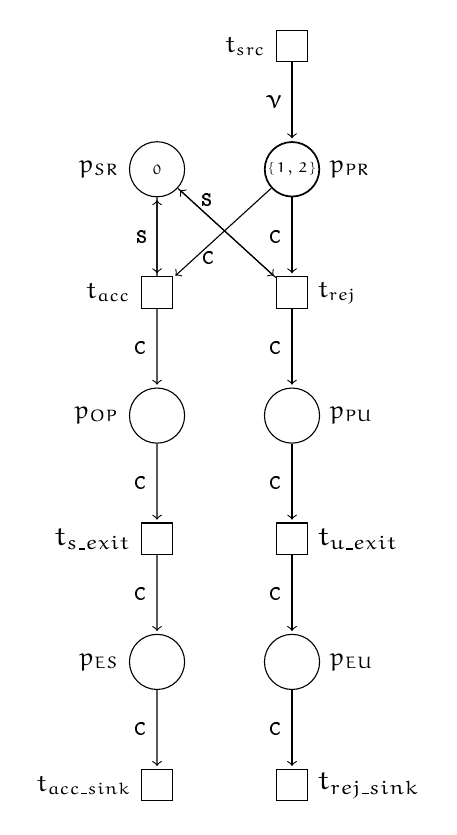
\begin{tikzpicture}[scale=0.7]
\centering

%source transition
\node[transition,minimum height=.4cm,minimum width=.4cm,label=left:{\small $t_{src}$}] (t0) {};

		
%parking requested client place
\node[place,label=right:{\small $p_{PR}$},minimum height=.70cm, minimum width=.5cm,below=of t0] (p0) {} 
edge[pre] node[auto] {$\nu$} (t0);
\node[token,fill = white, minimum height=0.40cm, minimum width=.5cm,draw=black,text=black] at (p0) {\text{$\{1,2\}$}};
		
		%server ready place			
		\node[place,label=left:{\small $p_{SR}$},minimum height=.70cm, minimum width=.5cm,left=of p0] (p1){};
\node[token,fill = white, text=black] at (p1) {$0$};

%places and transitions for request granted scenarios		
		%accept transition
		\node[transition,minimum height=.4cm,minimum width=.4cm,label=left:{\small $t_{acc}$}, below=of p1] (t1){}
		edge[pre] node[auto] {s} (p1)
		edge[post] node[auto] {} (p1)
		edge[pre] node[xshift=-5pt, yshift=-9pt] {c} (p0);
		%edge[post] node[auto] {} (p0);
		
	
		%client place occupy parking lot op
		\node[place,label=left:{\small $p_{OP}$},minimum height=.70cm, minimum width=.5cm,below=of t1] (p2){}
		edge[pre] node[auto] {c} (t1) ;	
		

		%transition exit successfully
		\node[transition,minimum height=.4cm,minimum width=.4cm,label=left:{$t_{s\_exit}$},below=of p2] (t2){}
		edge[pre] node[auto] {c} (p2);
		
		%client place Exit successfully ES
		\node[place,label=left:{\small $p_{ES}$},minimum height=.70cm, minimum width=.5cm,below=of t2] (p4){}
		edge[pre] node[auto] {c} (t2);			

		
		%transition accept sink
		\node[transition,minimum height=.4cm,minimum width=.4cm,label=left:{\small $t_{acc\_sink}$},below=of p4] (t3) {} edge[pre] node[auto] {c} (p4) ;
		
%request rejected scenarios		
		
		%reject transition
		\node[transition,minimum height=.4cm,minimum width=.4cm,label=right:{\small $t_{rej}$},below=of p0] (t4){}
		edge[pre] node[xshift=-7pt,yshift=12pt] {s} (p1)
		edge[post] node[auto] {} (p1)
		edge[pre] node[auto] {c} (p0);
		%edge[post] node[auto] {} (p0);


		%client place parking unavailable PU
		\node[place,label=right:{\small $p_{PU}$},minimum height=.70cm, minimum width=.5cm,below=of t4] (p6){}
		edge[pre] node[auto] {c} (t4) ;

		% transition unsuccesful exit
		\node[transition,minimum height=.4cm,minimum width=.4cm,label=right:{$t_{u\_exit}$},below= of p6] (t5) {}
		edge[pre] node[auto] {c} (p6);

		%client place Exit unsuccessfully EU
		\node[place,label=right:{\small $p_{EU}$},minimum height=.70cm, minimum width=.5cm,below=of t5] (p7){}
		edge[pre] node[auto] {c} (t5) ;

		% transition reject sink
		\node[transition,minimum height=.4cm,minimum width=.4cm,label=right:{$t_{rej\_sink}$},below= of p7] (t5) {}
		edge[pre] node[auto] {c} (p7);


\end{tikzpicture}


}
\end{figure}   
\end{column}
\end{columns} 
\end{frame}

\begin{frame}{Parking system as a $\nu$-net}
\begin{columns}
\begin{column}{.6\textwidth}
 A $\nu$-net is a labelled coloured Petri Net $N=(P,T,F,\lambda)$, where 
\begin{itemize} 
\item $P$ and $T$ are finite disjoint sets of places and transitions of the net, respectively,
\item $F$: $(P \times T) \cup (T \times P) \to \mathcal{MS(\text{Var})}$ defines the set of arcs of the net. 
\item $\lambda:~T\to Sync$ is a function labelling transitions.
\begin{itemize}
    \item [-] $\nu \not \in pre(t)$ for every $t \in T$ where
    \item [-] $pre(t)=\bigcup_{p\in P} S(F(p,t))$
    \item [-] $post(t)=\bigcup_{p\in P} S(F(t,p))$
    \item [-] $Var= pre(t) \bigcup post(t)$
\end{itemize}

\end{itemize} 
\end{column}
\begin{column}{.4\textwidth}
\begin{figure}[!ht]
\centering
\scalebox{0.7}{\usetikzlibrary {petri,positioning}
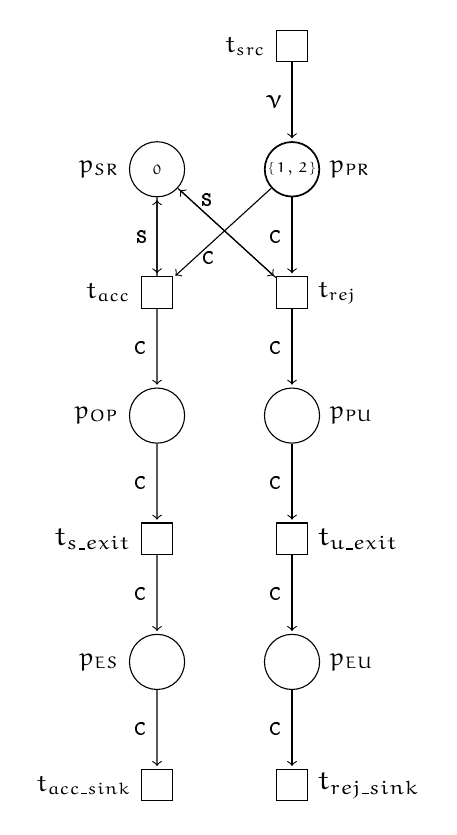
\begin{tikzpicture}[scale=0.7]
\centering

%source transition
\node[transition,minimum height=.4cm,minimum width=.4cm,label=left:{\small $t_{src}$}] (t0) {};

		
%parking requested client place
\node[place,label=right:{\small $p_{PR}$},minimum height=.70cm, minimum width=.5cm,below=of t0] (p0) {} 
edge[pre] node[auto] {$\nu$} (t0);
\node[token,fill = white, minimum height=0.40cm, minimum width=.5cm,draw=black,text=black] at (p0) {\text{$\{1,2\}$}};
		
		%server ready place			
		\node[place,label=left:{\small $p_{SR}$},minimum height=.70cm, minimum width=.5cm,left=of p0] (p1){};
\node[token,fill = white, text=black] at (p1) {$0$};

%places and transitions for request granted scenarios		
		%accept transition
		\node[transition,minimum height=.4cm,minimum width=.4cm,label=left:{\small $t_{acc}$}, below=of p1] (t1){}
		edge[pre] node[auto] {s} (p1)
		edge[post] node[auto] {} (p1)
		edge[pre] node[xshift=-5pt, yshift=-9pt] {c} (p0);
		%edge[post] node[auto] {} (p0);
		
	
		%client place occupy parking lot op
		\node[place,label=left:{\small $p_{OP}$},minimum height=.70cm, minimum width=.5cm,below=of t1] (p2){}
		edge[pre] node[auto] {c} (t1) ;	
		

		%transition exit successfully
		\node[transition,minimum height=.4cm,minimum width=.4cm,label=left:{$t_{s\_exit}$},below=of p2] (t2){}
		edge[pre] node[auto] {c} (p2);
		
		%client place Exit successfully ES
		\node[place,label=left:{\small $p_{ES}$},minimum height=.70cm, minimum width=.5cm,below=of t2] (p4){}
		edge[pre] node[auto] {c} (t2);			

		
		%transition accept sink
		\node[transition,minimum height=.4cm,minimum width=.4cm,label=left:{\small $t_{acc\_sink}$},below=of p4] (t3) {} edge[pre] node[auto] {c} (p4) ;
		
%request rejected scenarios		
		
		%reject transition
		\node[transition,minimum height=.4cm,minimum width=.4cm,label=right:{\small $t_{rej}$},below=of p0] (t4){}
		edge[pre] node[xshift=-7pt,yshift=12pt] {s} (p1)
		edge[post] node[auto] {} (p1)
		edge[pre] node[auto] {c} (p0);
		%edge[post] node[auto] {} (p0);


		%client place parking unavailable PU
		\node[place,label=right:{\small $p_{PU}$},minimum height=.70cm, minimum width=.5cm,below=of t4] (p6){}
		edge[pre] node[auto] {c} (t4) ;

		% transition unsuccesful exit
		\node[transition,minimum height=.4cm,minimum width=.4cm,label=right:{$t_{u\_exit}$},below= of p6] (t5) {}
		edge[pre] node[auto] {c} (p6);

		%client place Exit unsuccessfully EU
		\node[place,label=right:{\small $p_{EU}$},minimum height=.70cm, minimum width=.5cm,below=of t5] (p7){}
		edge[pre] node[auto] {c} (t5) ;

		% transition reject sink
		\node[transition,minimum height=.4cm,minimum width=.4cm,label=right:{$t_{rej\_sink}$},below= of p7] (t5) {}
		edge[pre] node[auto] {c} (p7);


\end{tikzpicture}


}
\end{figure}   
\end{column}
\end{columns} 
\end{frame}




\begin{frame}{Parking system as a $\nu$-net}
\begin{columns}
\begin{column}{.6\textwidth}
\begin{itemize}
\item A marking  of a $\nu$-net $N=(P,T,F,\lambda)$ is a function $M:P\to(MS(Id))$
\item We denote by $S(M)$ the set of names in $M$. i.e, $S(M)=\bigcup_{p\in P}S(M(p))$.
\item If $t$ is an \colorbox{green!30}{autonomous transition} then it must be the case that every variable annotating a postcondition arc, except $\nu$, also annotates some precondition arc in the net.
\end{itemize}
\end{column}
\begin{column}{.4\textwidth}
\begin{figure}[!ht]
\centering
\scalebox{0.7}{\usetikzlibrary {petri,positioning}
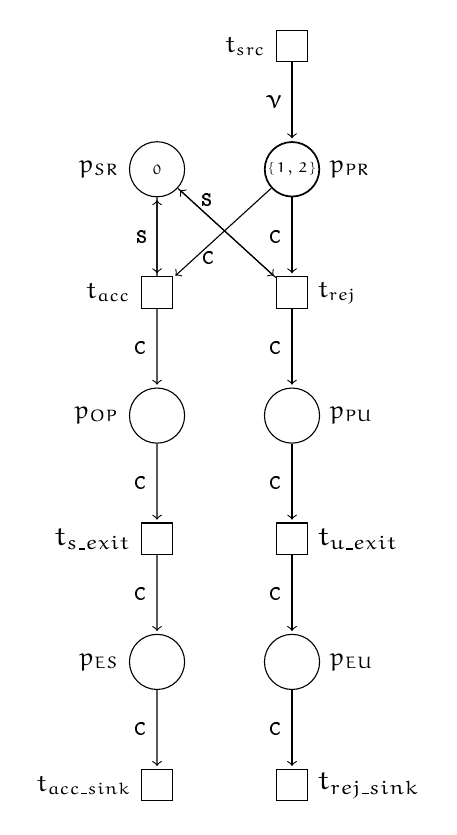
\begin{tikzpicture}[scale=0.7]
\centering

%source transition
\node[transition,minimum height=.4cm,minimum width=.4cm,label=left:{\small $t_{src}$}] (t0) {};

		
%parking requested client place
\node[place,label=right:{\small $p_{PR}$},minimum height=.70cm, minimum width=.5cm,below=of t0] (p0) {} 
edge[pre] node[auto] {$\nu$} (t0);
\node[token,fill = white, minimum height=0.40cm, minimum width=.5cm,draw=black,text=black] at (p0) {\text{$\{1,2\}$}};
		
		%server ready place			
		\node[place,label=left:{\small $p_{SR}$},minimum height=.70cm, minimum width=.5cm,left=of p0] (p1){};
\node[token,fill = white, text=black] at (p1) {$0$};

%places and transitions for request granted scenarios		
		%accept transition
		\node[transition,minimum height=.4cm,minimum width=.4cm,label=left:{\small $t_{acc}$}, below=of p1] (t1){}
		edge[pre] node[auto] {s} (p1)
		edge[post] node[auto] {} (p1)
		edge[pre] node[xshift=-5pt, yshift=-9pt] {c} (p0);
		%edge[post] node[auto] {} (p0);
		
	
		%client place occupy parking lot op
		\node[place,label=left:{\small $p_{OP}$},minimum height=.70cm, minimum width=.5cm,below=of t1] (p2){}
		edge[pre] node[auto] {c} (t1) ;	
		

		%transition exit successfully
		\node[transition,minimum height=.4cm,minimum width=.4cm,label=left:{$t_{s\_exit}$},below=of p2] (t2){}
		edge[pre] node[auto] {c} (p2);
		
		%client place Exit successfully ES
		\node[place,label=left:{\small $p_{ES}$},minimum height=.70cm, minimum width=.5cm,below=of t2] (p4){}
		edge[pre] node[auto] {c} (t2);			

		
		%transition accept sink
		\node[transition,minimum height=.4cm,minimum width=.4cm,label=left:{\small $t_{acc\_sink}$},below=of p4] (t3) {} edge[pre] node[auto] {c} (p4) ;
		
%request rejected scenarios		
		
		%reject transition
		\node[transition,minimum height=.4cm,minimum width=.4cm,label=right:{\small $t_{rej}$},below=of p0] (t4){}
		edge[pre] node[xshift=-7pt,yshift=12pt] {s} (p1)
		edge[post] node[auto] {} (p1)
		edge[pre] node[auto] {c} (p0);
		%edge[post] node[auto] {} (p0);


		%client place parking unavailable PU
		\node[place,label=right:{\small $p_{PU}$},minimum height=.70cm, minimum width=.5cm,below=of t4] (p6){}
		edge[pre] node[auto] {c} (t4) ;

		% transition unsuccesful exit
		\node[transition,minimum height=.4cm,minimum width=.4cm,label=right:{$t_{u\_exit}$},below= of p6] (t5) {}
		edge[pre] node[auto] {c} (p6);

		%client place Exit unsuccessfully EU
		\node[place,label=right:{\small $p_{EU}$},minimum height=.70cm, minimum width=.5cm,below=of t5] (p7){}
		edge[pre] node[auto] {c} (t5) ;

		% transition reject sink
		\node[transition,minimum height=.4cm,minimum width=.4cm,label=right:{$t_{rej\_sink}$},below= of p7] (t5) {}
		edge[pre] node[auto] {c} (p7);


\end{tikzpicture}


}
\end{figure}   
\end{column}
\end{columns} 
\end{frame}



\begin{frame}{Parking system as a $\nu$-net}
\begin{itemize}
\item A $\nu$-net system is a set of disjoint $\nu$-net components. $post,pre,Var$ are defined over the tuple of transitions in a net, by taking the union operation.
\item Let $\bar{t}=(t_1,\ldots, t_n)$ be a tuple of transitions of a $\nu$-net system. The transitions in $\bar{t}$ are \colorbox{green!30}{\emph{compatible}} if:
\begin{itemize}
    \item $\lambda(t_i)=s(i)$ for some $s\in S$ with $arity(s)=n$,
    \item $post(\bar{t})\setminus \{\nu\}\subseteq pre(\bar{t}$
\end{itemize}
\item A mode of a tuple of compatible transitions $\bar{t}$ is a mapping $\sigma:Var(\bar{t})\to Id$, instantiating every variable in the adjacent arcs of $\bar{t}$ to some identifier.
\item Let $N$ be a $\nu$-net system and $M$ a marking of $N$. We say that $M$ \colorbox{green!30}{enables} the tuple of transitions $\bar{t}$ with mode $\sigma$ whenever:

\begin{itemize}
    \item If $\nu \in Var(t)$ then $\sigma(\nu)\not \in S(M)$
    \item $\sigma(F(p,\bar{t}))\subseteq M(p)$ for all $p \in P$.
\end{itemize}


 
 \end{itemize}

\end{frame}


\begin{frame}{Parking system as a $\nu$-net}
\begin{itemize}
 \item The \colorbox{green!30}{reached marking} of $N$ after firing of $\bar{t}$ with mode $\sigma$ is denoted by $M \xrightarrow{\bar{t(\sigma)}}M'$
 \item[] $M'(p)=M(p) - \sigma(F(p,\bar{t})) + \sigma(F(\bar{t},p))$ for every $p \in P$.
 \item Notice the  $\sigma(\nu)\not \in S(M)$ for the enabling of transition, that causes the creation of fresh (equal) identifiers in all the places reached by arcs labelled by the special variable $\nu$.

 \item Since $F(p,\bar{t})$ and $F(\bar{t},p)$ are both multisets of variables, and $\sigma$ maps variables to identifiers, $\sigma(F(p,\bar{t}))$ and $\sigma(F(\bar{t},p))$ are \colorbox{green!30} {both multisets of identifiers}, that can be removed from, added to $M(p)$.
 \end{itemize}

\end{frame}



\begin{frame}{Requirements in the formal model}
\begin{enumerate}
    \item We want \sout{tokens} \colorbox{green!30}{identifiers} for the processes
    \item Distinguish between the \colorbox{green!30}{client process (identifiers)} and \colorbox{green!30}{server process}
    \item Dynamically create an \colorbox{green!30}{unbounded number} of client identifiers (a finite number of clients at any marking)
    \item \colorbox{green!30}{Purge client identifiers} when clients die (no re-use of identifiers)
    \item Server process is immortal
    \item Communication: 
    \begin{itemize}
        \item Server-client interaction exists.
        \item No communication among clients. 
    \end{itemize}
    \item \colorbox{red!30}{How do we handle synchronizations and forks?}
\end{enumerate}    
\end{frame}


\begin{frame}{Requirements for the formal model (Answered)}
\begin{enumerate}
    \item Instead of tokens, we want \colorbox{green!30}{identifiers} for the processes
    \item[] \textcolor{purple}{Colored Petri net (side note: CPN Tools - broken toolchain, CPN ML is overkill!)}
    \item Distinguish between the \colorbox{green!30}{client process (identifiers)} and \colorbox{green!30}{server process}
    \item[] \textcolor{purple}{Server process has id $0$, client identifiers range over $\{\mathbb{N}\setminus 0\}$}
    \item Dynamically create an \colorbox{green!30}{unbounded number} of client identifiers (a finite number of clients at any marking)
    \item[] \textcolor{purple}{Post-condition arcs labeled $\nu$}
    \item \colorbox{green!30}{Purge client identifiers} when clients die (no re-use of identifiers)
    \item[] \textcolor{purple}{Ensured by sink transition and $\nu$-arcs}
   
\end{enumerate}    
\end{frame}


\begin{frame}{Requirements in the formal model (Answered)}
\begin{enumerate}
\setcounter{enumi}{4}
 \item Server process is immortal
 \item[] \textcolor{purple}{Ensured by the structure of the net}
 \item Communication: 
    \begin{itemize}
        \item Server-client interaction exists.
        \item No communication among clients. 
    \end{itemize}
 \item[] \textcolor{purple}{Ensured by the structure of the net}
 \item \colorbox{red!30}{How do we handle synchronizations and forks?}
 \item[] \textcolor{purple}{using the semantics of the $\nu$-net}
\end{enumerate}    
\end{frame}


\begin{frame}{}
    \centering    
    \huge{Question: What is a suitable\footnote[1]{satisfying the above requirements} formal model for the system?}
    \textcolor{purple}{restricted $\nu$-nets}
\end{frame}



\begin{frame}{Introducing restricted $\nu$-nets}
\begin{itemize}
    \item $S$ is a set of service names, with function $arity: S\to \mathbb{N}$
     \item Distinguishable tokens taken from an arbitrary infinite set Id
    \item A finite set of variables $Var$
    \item Arcs are labeled by $v \in Var$.
    \item Create fresh names using a special variable $\nu \in Var$ that appears only in post condition arcs
\end{itemize}   
\end{frame}


\begin{frame}{Parking system as a restricted $\nu$-net}
 
 A restricted $\nu$-net is a labelled coloured Petri Net $N=(P,T,F)$, where 
\begin{itemize} 
\item $P$ and $T$ are finite disjoint sets of places and transitions of the net, respectively,
\item $F$: $(P \times T) \cup (T \times P) \to \mathcal{MS(\text{Var})}$ defines the set of arcs of the net. 
%\item $\lambda:~T\to Sync$ is a function labelling transitions.
\begin{itemize}
    \item [-] $\nu \not \in pre(t)$ for every $t \in T$ where
    \item [-] $pre(t)=\bigcup_{p\in P} S(F(p,t))$
    \item [-] $post(t)=\bigcup_{p\in P} S(F(t,p))$
    \item [-] $Var= pre(t) \bigcup post(t)$
\end{itemize}
\item Notice that $\nu$-net contains a function labelling transitions $\lambda$, which are useful for synchronization between components. This is absent in the restricted $\nu$-net that we consider here.
\end{itemize} 

\end{frame}




\begin{frame}{Parking system as a restricted $\nu$-net}

\begin{itemize}
\item A marking  of a restricted $\nu$-net $N=(P,T,F)$ is a function $M:P\to(MS(Id))$
\item We denote by $S(M)$ the set of names in $M$. i.e, $S(M)=\bigcup_{p\in P}S(M(p))$.

\end{itemize}
\end{frame}



\begin{frame}{Parking system as a restricted $\nu$-net}
\begin{itemize}
\item A transition is said to be \colorbox{green!30}{\emph{identifier-preserving}} if the following condition holds:\begin{itemize}
    \item $post(t)\setminus \{\nu\}\subseteq pre(t)$
\end{itemize}
\item A mode of a transition $t$ is a mapping $\sigma:Var(t)\to Id$, instantiating every variable in the adjacent arcs of $t$ to some identifier.
\item \textbf{Enabledness rule: }Let $N$ be a restricted $\nu$-net and $M$ a marking of $N$. We say that $M$ \colorbox{green!30}{enables} the transition $t$ with mode $\sigma$ whenever:

\begin{itemize}
    \item If $\nu \in Var(t)$ then $\sigma(\nu)\not \in S(M)$
    \item $\sigma(F(p,t))\subseteq M(p)$ for all $p \in P$.
\end{itemize}


 
 \end{itemize}

\end{frame}


\begin{frame}{Parking system as a restricted $\nu$-net}
\begin{itemize}
 \item The \colorbox{green!30}{reached marking} of $N$ after firing of $t$ with mode $\sigma$ is denoted by $M \xrightarrow{t(\sigma)}M'$
 \item[] $M'(p)=M(p) - \sigma(F(p,t)) + \sigma(F(t,p))$ for every $p \in P$.
 \item Notice the  $\sigma(\nu)\not \in S(M)$ for the enabling of transition, that causes the creation of fresh (equal) identifiers in all the places reached by arcs labelled by the special variable $\nu$.

 \item Since $F(p,t)$ and $F(t,p)$ are both multisets of variables, and $\sigma$ maps variables to identifiers, $\sigma(F(p,t))$ and $\sigma(F(t,p))$ are \colorbox{green!30} {both multisets of identifiers}, that can be removed from, added to $M(p)$.
 \end{itemize}

\end{frame}
\end{comment}


\end{document}